

\tikzset{every picture/.style={line width=0.75pt}} %set default line width to 0.75pt        

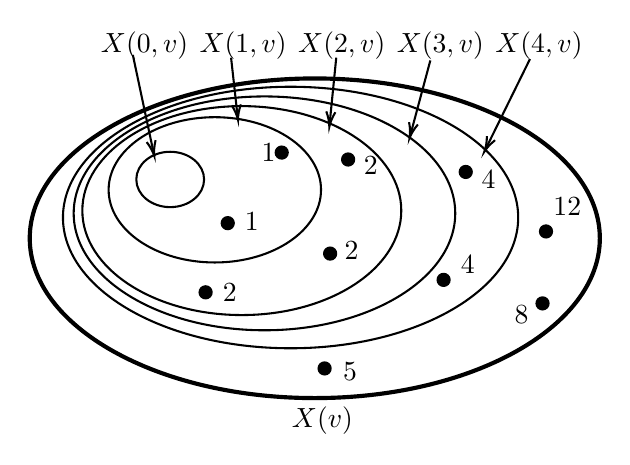
\begin{tikzpicture}[x=0.5pt,y=0.5pt,yscale=-1,xscale=1]
%uncomment if require: \path (0,327); %set diagram left start at 0, and has height of 327

%Shape: Ellipse [id:dp0428766556986383] 
\draw  [line width=1.5]  (59,177.5) .. controls (59,113.71) and (151.23,62) .. (265,62) .. controls (378.77,62) and (471,113.71) .. (471,177.5) .. controls (471,241.29) and (378.77,293) .. (265,293) .. controls (151.23,293) and (59,241.29) .. (59,177.5) -- cycle ;
%Shape: Ellipse [id:dp14451946279796424] 
\draw   (136,135) .. controls (136,123.95) and (146.97,115) .. (160.5,115) .. controls (174.03,115) and (185,123.95) .. (185,135) .. controls (185,146.05) and (174.03,155) .. (160.5,155) .. controls (146.97,155) and (136,146.05) .. (136,135) -- cycle ;
%Shape: Ellipse [id:dp2511588613225232] 
\draw   (116,142.5) .. controls (116,113.51) and (150.36,90) .. (192.75,90) .. controls (235.14,90) and (269.5,113.51) .. (269.5,142.5) .. controls (269.5,171.49) and (235.14,195) .. (192.75,195) .. controls (150.36,195) and (116,171.49) .. (116,142.5) -- cycle ;
%Shape: Ellipse [id:dp5415787744293407] 
\draw   (97,157.5) .. controls (97,115.8) and (148.6,82) .. (212.25,82) .. controls (275.9,82) and (327.5,115.8) .. (327.5,157.5) .. controls (327.5,199.2) and (275.9,233) .. (212.25,233) .. controls (148.6,233) and (97,199.2) .. (97,157.5) -- cycle ;
%Shape: Ellipse [id:dp42014218433161865] 
\draw   (83,162.5) .. controls (83,110.31) and (156.65,68) .. (247.5,68) .. controls (338.35,68) and (412,110.31) .. (412,162.5) .. controls (412,214.69) and (338.35,257) .. (247.5,257) .. controls (156.65,257) and (83,214.69) .. (83,162.5) -- cycle ;
%Flowchart: Connector [id:dp24980663040863116] 
\draw  [fill={rgb, 255:red, 0; green, 0; blue, 0 }  ,fill opacity=1 ] (198,165) .. controls (198.87,162.74) and (201.4,161.62) .. (203.66,162.49) .. controls (205.91,163.36) and (207.04,165.89) .. (206.17,168.15) .. controls (205.3,170.4) and (202.77,171.53) .. (200.51,170.66) .. controls (198.26,169.79) and (197.13,167.26) .. (198,165) -- cycle ;
%Flowchart: Connector [id:dp6930751898796546] 
\draw  [fill={rgb, 255:red, 0; green, 0; blue, 0 }  ,fill opacity=1 ] (237,114) .. controls (237.87,111.74) and (240.4,110.62) .. (242.66,111.49) .. controls (244.91,112.36) and (246.04,114.89) .. (245.17,117.15) .. controls (244.3,119.4) and (241.77,120.53) .. (239.51,119.66) .. controls (237.26,118.79) and (236.13,116.26) .. (237,114) -- cycle ;
%Flowchart: Connector [id:dp6974875632568183] 
\draw  [fill={rgb, 255:red, 0; green, 0; blue, 0 }  ,fill opacity=1 ] (425.5,223) .. controls (426.37,220.74) and (428.9,219.62) .. (431.16,220.49) .. controls (433.41,221.36) and (434.54,223.89) .. (433.67,226.15) .. controls (432.8,228.4) and (430.27,229.53) .. (428.01,228.66) .. controls (425.76,227.79) and (424.63,225.26) .. (425.5,223) -- cycle ;
%Flowchart: Connector [id:dp15058432994873683] 
\draw  [fill={rgb, 255:red, 0; green, 0; blue, 0 }  ,fill opacity=1 ] (182,215) .. controls (182.87,212.74) and (185.4,211.62) .. (187.66,212.49) .. controls (189.91,213.36) and (191.04,215.89) .. (190.17,218.15) .. controls (189.3,220.4) and (186.77,221.53) .. (184.51,220.66) .. controls (182.26,219.79) and (181.13,217.26) .. (182,215) -- cycle ;
%Flowchart: Connector [id:dp1384061319550981] 
\draw  [fill={rgb, 255:red, 0; green, 0; blue, 0 }  ,fill opacity=1 ] (428,171) .. controls (428.87,168.74) and (431.4,167.62) .. (433.66,168.49) .. controls (435.91,169.36) and (437.04,171.89) .. (436.17,174.15) .. controls (435.3,176.4) and (432.77,177.53) .. (430.51,176.66) .. controls (428.26,175.79) and (427.13,173.26) .. (428,171) -- cycle ;
%Flowchart: Connector [id:dp9185176159520061] 
\draw  [fill={rgb, 255:red, 0; green, 0; blue, 0 }  ,fill opacity=1 ] (354,206) .. controls (354.87,203.74) and (357.4,202.62) .. (359.66,203.49) .. controls (361.91,204.36) and (363.04,206.89) .. (362.17,209.15) .. controls (361.3,211.4) and (358.77,212.53) .. (356.51,211.66) .. controls (354.26,210.79) and (353.13,208.26) .. (354,206) -- cycle ;
%Flowchart: Connector [id:dp9264926624537071] 
\draw  [fill={rgb, 255:red, 0; green, 0; blue, 0 }  ,fill opacity=1 ] (370,128) .. controls (370.87,125.74) and (373.4,124.62) .. (375.66,125.49) .. controls (377.91,126.36) and (379.04,128.89) .. (378.17,131.15) .. controls (377.3,133.4) and (374.77,134.53) .. (372.51,133.66) .. controls (370.26,132.79) and (369.13,130.26) .. (370,128) -- cycle ;
%Flowchart: Connector [id:dp8504406787781214] 
\draw  [fill={rgb, 255:red, 0; green, 0; blue, 0 }  ,fill opacity=1 ] (272,187) .. controls (272.87,184.74) and (275.4,183.62) .. (277.66,184.49) .. controls (279.91,185.36) and (281.04,187.89) .. (280.17,190.15) .. controls (279.3,192.4) and (276.77,193.53) .. (274.51,192.66) .. controls (272.26,191.79) and (271.13,189.26) .. (272,187) -- cycle ;
%Flowchart: Connector [id:dp2675280100573806] 
\draw  [fill={rgb, 255:red, 0; green, 0; blue, 0 }  ,fill opacity=1 ] (285,119) .. controls (285.87,116.74) and (288.4,115.62) .. (290.66,116.49) .. controls (292.91,117.36) and (294.04,119.89) .. (293.17,122.15) .. controls (292.3,124.4) and (289.77,125.53) .. (287.51,124.66) .. controls (285.26,123.79) and (284.13,121.26) .. (285,119) -- cycle ;
%Flowchart: Connector [id:dp5988515924155521] 
\draw  [fill={rgb, 255:red, 0; green, 0; blue, 0 }  ,fill opacity=1 ] (268,270) .. controls (268.87,267.74) and (271.4,266.62) .. (273.66,267.49) .. controls (275.91,268.36) and (277.04,270.89) .. (276.17,273.15) .. controls (275.3,275.4) and (272.77,276.53) .. (270.51,275.66) .. controls (268.26,274.79) and (267.13,272.26) .. (268,270) -- cycle ;
%Straight Lines [id:da885882466037084] 
\draw    (133.5,45) -- (148.58,116.04) ;
\draw [shift={(149,118)}, rotate = 258.01] [color={rgb, 255:red, 0; green, 0; blue, 0 }  ][line width=0.75]    (10.93,-3.29) .. controls (6.95,-1.4) and (3.31,-0.3) .. (0,0) .. controls (3.31,0.3) and (6.95,1.4) .. (10.93,3.29)   ;
%Straight Lines [id:da07374180723453116] 
\draw    (204.5,47) -- (209.28,90.01) ;
\draw [shift={(209.5,92)}, rotate = 263.65999999999997] [color={rgb, 255:red, 0; green, 0; blue, 0 }  ][line width=0.75]    (10.93,-3.29) .. controls (6.95,-1.4) and (3.31,-0.3) .. (0,0) .. controls (3.31,0.3) and (6.95,1.4) .. (10.93,3.29)   ;
%Straight Lines [id:da8157366219842463] 
\draw    (280.5,47) -- (275.7,95.01) ;
\draw [shift={(275.5,97)}, rotate = 275.71] [color={rgb, 255:red, 0; green, 0; blue, 0 }  ][line width=0.75]    (10.93,-3.29) .. controls (6.95,-1.4) and (3.31,-0.3) .. (0,0) .. controls (3.31,0.3) and (6.95,1.4) .. (10.93,3.29)   ;
%Straight Lines [id:da939078987537615] 
\draw    (348.5,49) -- (334.02,103.07) ;
\draw [shift={(333.5,105)}, rotate = 285] [color={rgb, 255:red, 0; green, 0; blue, 0 }  ][line width=0.75]    (10.93,-3.29) .. controls (6.95,-1.4) and (3.31,-0.3) .. (0,0) .. controls (3.31,0.3) and (6.95,1.4) .. (10.93,3.29)   ;
%Shape: Ellipse [id:dp10244037755425861] 
\draw   (90.75,159.5) .. controls (90.75,112.83) and (152.48,75) .. (228.63,75) .. controls (304.77,75) and (366.5,112.83) .. (366.5,159.5) .. controls (366.5,206.17) and (304.77,244) .. (228.63,244) .. controls (152.48,244) and (90.75,206.17) .. (90.75,159.5) -- cycle ;
%Straight Lines [id:da2534194459074104] 
\draw    (420.5,48) -- (388.38,113.21) ;
\draw [shift={(387.5,115)}, rotate = 296.22] [color={rgb, 255:red, 0; green, 0; blue, 0 }  ][line width=0.75]    (10.93,-3.29) .. controls (6.95,-1.4) and (3.31,-0.3) .. (0,0) .. controls (3.31,0.3) and (6.95,1.4) .. (10.93,3.29)   ;

% Text Node
\draw (212.24,157.06) node [anchor=north west][inner sep=0.75pt]   [align=left] {$\displaystyle 1$};
% Text Node
\draw (224.24,107.06) node [anchor=north west][inner sep=0.75pt]   [align=left] {$\displaystyle 1$};
% Text Node
\draw (196.24,208.06) node [anchor=north west][inner sep=0.75pt]   [align=left] {$\displaystyle 2$};
% Text Node
\draw (284.24,178.06) node [anchor=north west][inner sep=0.75pt]   [align=left] {$\displaystyle 2$};
% Text Node
\draw (298.24,116.06) node [anchor=north west][inner sep=0.75pt]   [align=left] {$\displaystyle 2$};
% Text Node
\draw (383.24,126.06) node [anchor=north west][inner sep=0.75pt]   [align=left] {$\displaystyle 4$};
% Text Node
\draw (368.24,188.06) node [anchor=north west][inner sep=0.75pt]   [align=left] {$\displaystyle 4$};
% Text Node
\draw (283.24,265.06) node [anchor=north west][inner sep=0.75pt]   [align=left] {$\displaystyle 5$};
% Text Node
\draw (407.24,224.06) node [anchor=north west][inner sep=0.75pt]   [align=left] {$\displaystyle 8$};
% Text Node
\draw (435.24,146.06) node [anchor=north west][inner sep=0.75pt]   [align=left] {$\displaystyle 12$};
% Text Node
\draw (108.24,26.06) node [anchor=north west][inner sep=0.75pt]   [align=left] {$\displaystyle X( 0,v)$};
% Text Node
\draw (179.49,26.06) node [anchor=north west][inner sep=0.75pt]   [align=left] {$\displaystyle X( 1,v)$};
% Text Node
\draw (250.74,26.06) node [anchor=north west][inner sep=0.75pt]   [align=left] {$\displaystyle X( 2,v)$};
% Text Node
\draw (393.24,26.06) node [anchor=north west][inner sep=0.75pt]   [align=left] {$\displaystyle X( 4,v)$};
% Text Node
\draw (246.24,297.06) node [anchor=north west][inner sep=0.75pt]   [align=left] {$\displaystyle X( v)$};
% Text Node
\draw (321.99,26.06) node [anchor=north west][inner sep=0.75pt]   [align=left] {$\displaystyle X( 3,v)$};


\end{tikzpicture}

